%<<<===
\subsection{Сохранение файла как *.tsv}

\begin{tcolorbox}
\begin{verbatim}
Меню:
1. Открыть файл
2. Ввод данных       
3. Вывод данных      
4. Сортирова по полю 
5. Удалить запись    
6. Сохранить как     
0. Выйти из программы
\end{verbatim}
\end{tcolorbox}

Для вывода таблицы в консоль, выбираю из меню пункт 3.

\begin{tcolorbox}
\begin{verbatim}
| ID   | байт Номер    | байт Марка    | байт Фамилия      | Осмотр     |
| ---- | ---- -------- | ---- -------- | ---- ------------ | ---------- |
| 0    | 8    m74y7d   | 10   Alpha    | 10   Podushkin    | Не пройден |
| 1    | 8    d4rh75   | 4    Ford     | 10   Kamerov      | Не пройден |
| 2    | 8    fruf45   | 3    BMW      | 10   Rozetkov     | Пройден    |
Нажмите любую клавишу для продолжения...
\end{verbatim}
\end{tcolorbox}

Чтобы вернуться в меню нажимаю любую клавишу.

\begin{tcolorbox}
\begin{verbatim}
Меню:
1. Открыть файл
2. Ввод данных       
3. Вывод данных      
4. Сортирова по полю 
5. Удалить запись    
6. Сохранить как     
0. Выйти из программы
\end{verbatim}
\end{tcolorbox}

Попал в главное меню. Чтобы сохранить файл, выбираю пункт 6.

\begin{tcolorbox}
\begin{verbatim}
Меню:
1. Сохранить как tsv файл
2. Сохранить как bin файл
0. Выйти
\end{verbatim}
\end{tcolorbox}

Появилось меню. Так как нужно сохранить в *.tsv формате, то выбираю пункт 1. TSV - Tab Separated Values файл. Это файл как таблица. Открыть таблицу можно, например, в Libre Office Calc (Скриншот на рисунке \ref{fig:data-tsv}). Также можно такие файлы просматривать на GitHub (Скриншот на рисунке \ref{fig:data-tsv-on-github}).

\begin{figure}[p]
    \center{
        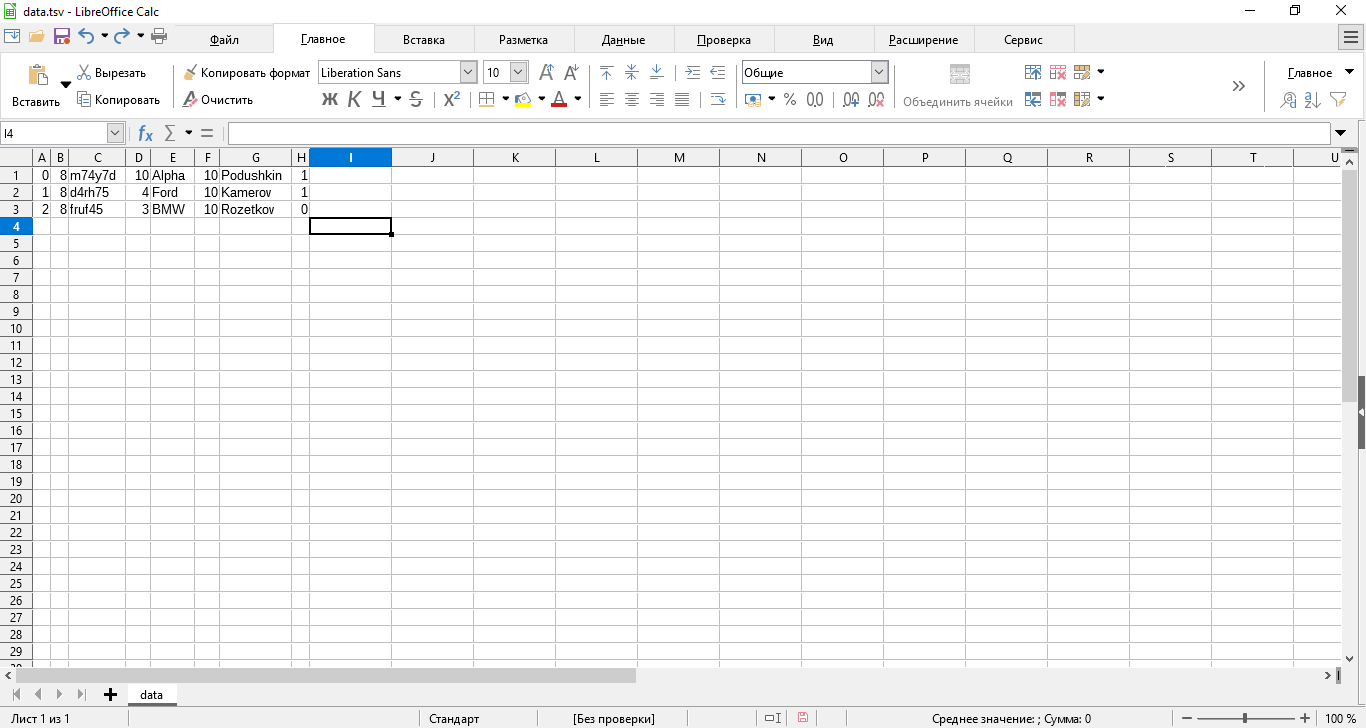
\includegraphics[width=16cm]{../pics/data-tsv-on-libre-office-calc.png}
    }
    \caption{data.tsv}
    \label{fig:data-tsv}
\end{figure}

\begin{figure}[p]
    \center{
        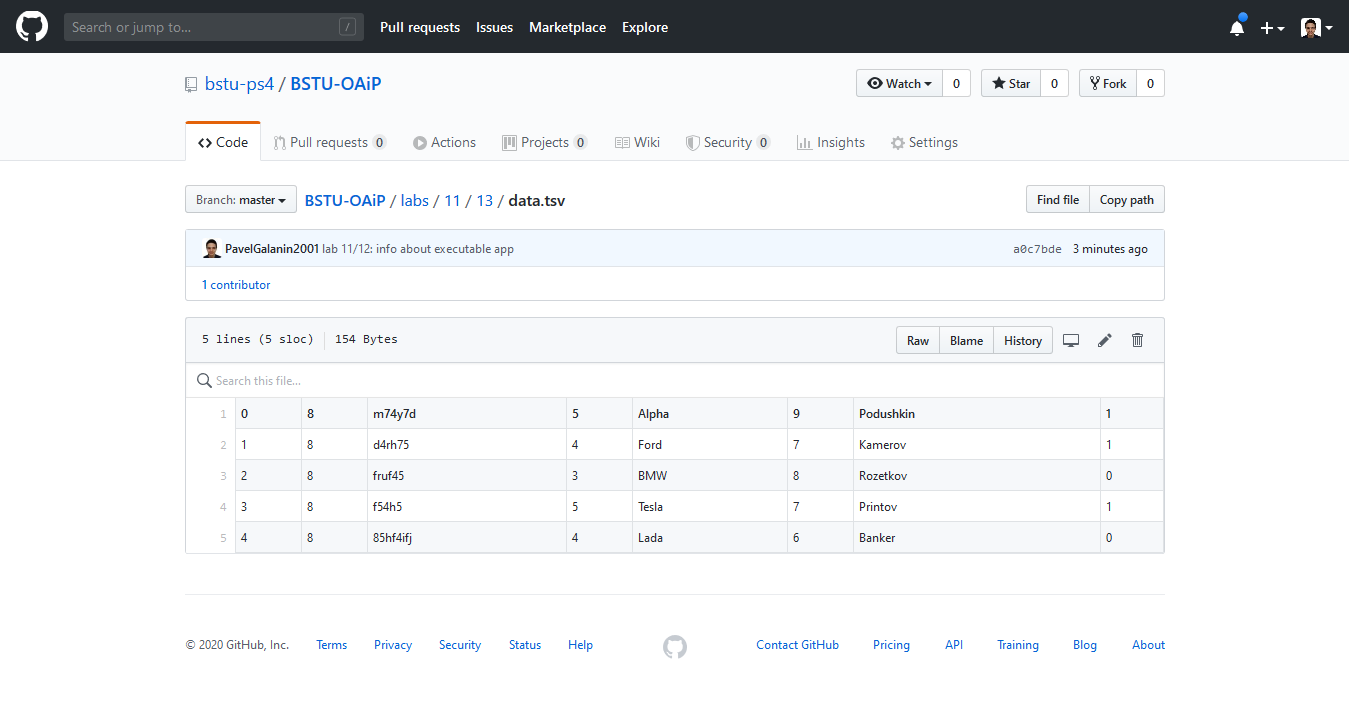
\includegraphics[width=16cm]{../pics/data-tsv-on-github.png}
    }
    \caption{data.tsv}
    \label{fig:data-tsv-on-github}
\end{figure}

Если открыть файл data.tsv, то там видем, что всё через табуляцию:
\begin{tcolorbox}
\begin{verbatim}
0	8	m74y7d	10	Alpha	10	Podushkin	1
1	8	d4rh75	4	Ford	10	Kamerov	1
2	8	fruf45	3	BMW	10	Rozetkov	0
\end{verbatim}
\end{tcolorbox}
%===>>>

\newpage

%<<<===
\subsection{Сохранение файла как *.bin}

\begin{tcolorbox}
\begin{verbatim}
Меню:
1. Открыть файл
2. Ввод данных
3. Вывод данных
4. Сортирова по полю
5. Удалить запись
6. Сохранить как
0. Выйти из программы
\end{verbatim}
\end{tcolorbox}

Для вывода таблицы в консоль, выбираю из меню пункт 3.
\begin{tcolorbox}
\begin{verbatim}
| ID   | байт Номер    | байт Марка    | байт Фамилия      | Осмотр     |
| ---- | ---- -------- | ---- -------- | ---- ------------ | ---------- |
| 0    | 8    m74y7d   | 5    Alpha    | 9    Podushkin    | Не пройден |
| 1    | 8    d4rh75   | 4    Ford     | 7    Kamerov      | Не пройден |
| 2    | 8    fruf45   | 3    BMW      | 8    Rozetkov     | Пройден    |
| 3    | 8    f54h5    | 5    Tesla    | 7    Printov      | Не пройден |
| 4    | 8    85hf4ifj | 4    Lada     | 6    Banker       | Пройден    |
Нажмите любую клавишу для продолжения...
\end{verbatim}
\end{tcolorbox}

Для выхода в меню, жму любую клавишу.

Попадаю в главное меню. Для сохранения файла, выбираю пункт 6.

\begin{tcolorbox}
\begin{verbatim}
Меню:
1. Сохранить как tsv файл
2. Сохранить как bin файл
0. Выйти
\end{verbatim}
\end{tcolorbox}

Появилось меню. Для сохранения в формате bin файла, выбираю пункт 2.

Появился файл data.bin (рисунок \ref{fig:far_folder}).

\begin{figure}[p]
    \center{
        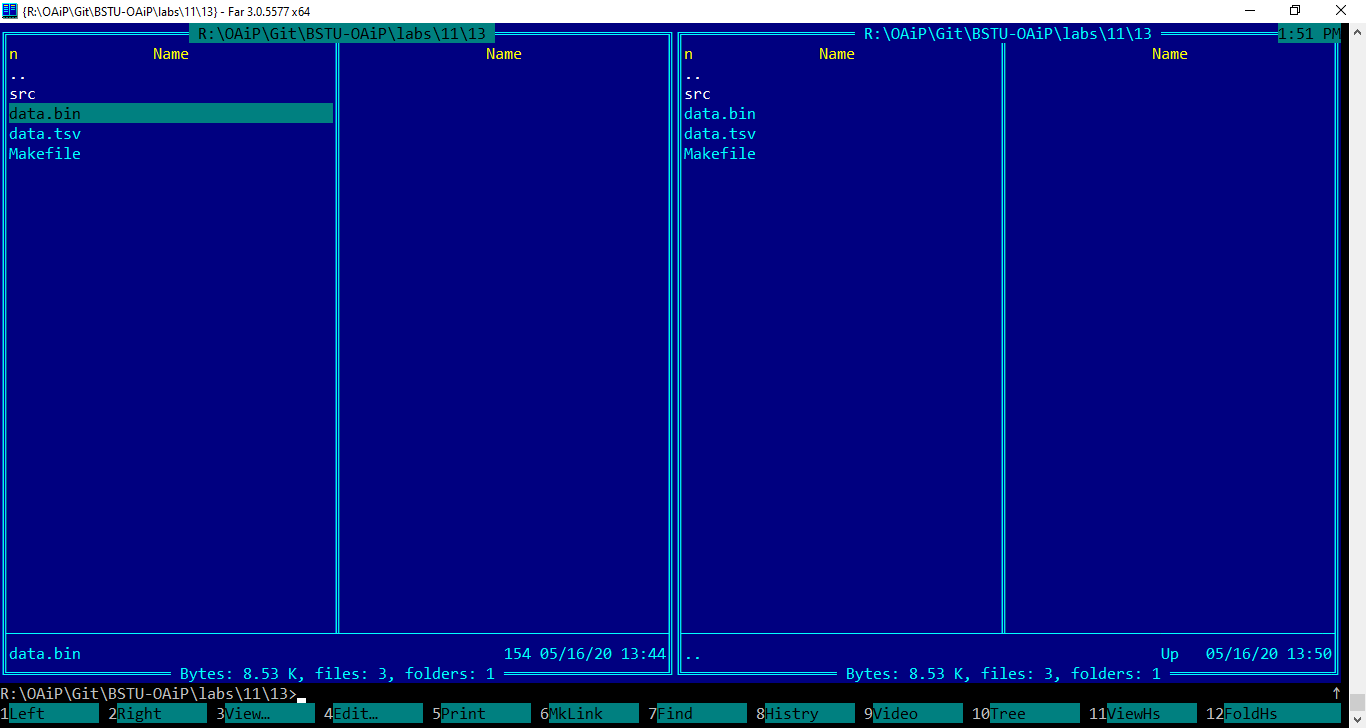
\includegraphics[width=16cm]{../pics/far-folder.png}
    }
    \caption{Бинарный файл в папке в Far Manager}
    \label{fig:far_folder}
\end{figure}

Открываю файл по нажатию F3. Видем как сохранился файл на рисунке \ref{fig:far_data_bin}.

\begin{figure}[p]
    \center{
        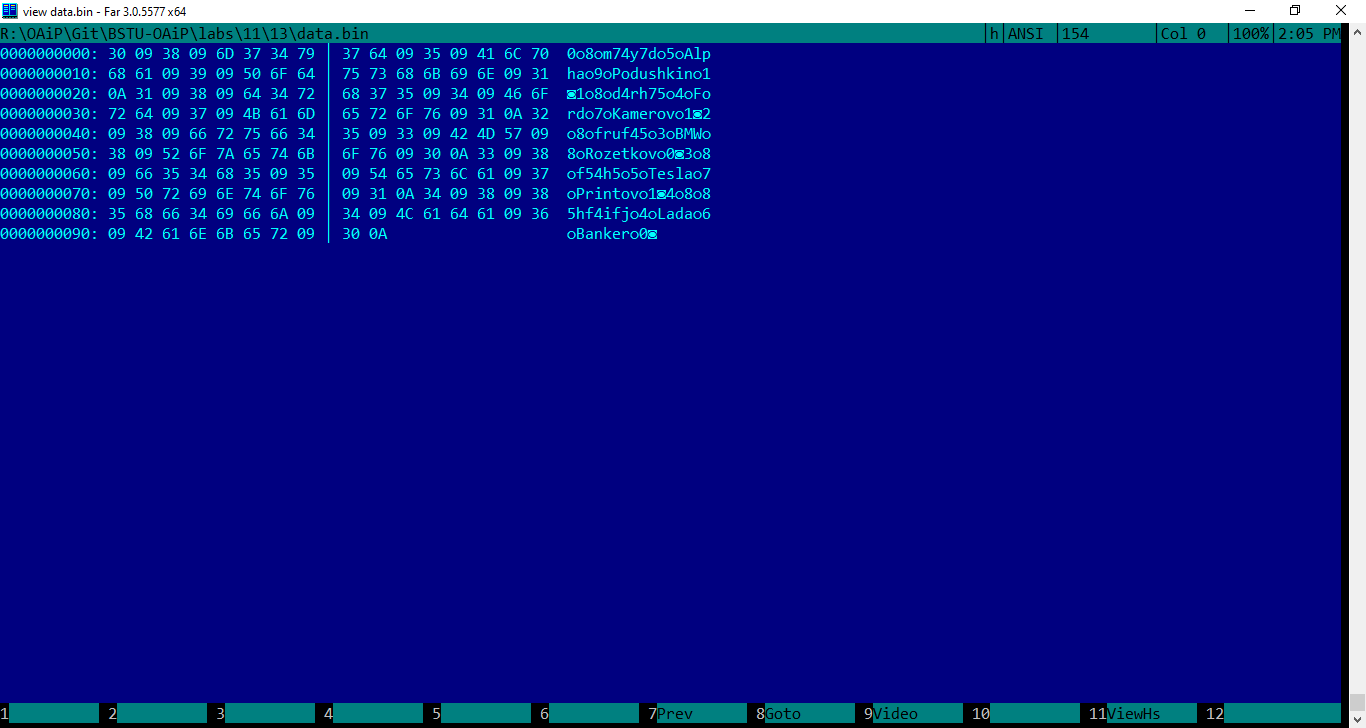
\includegraphics[width=16cm]{../pics/far-data-bin.png}
    }
    \caption{Бинарный файл в открытый по F3 в Far Manager}
    \label{fig:far_data_bin}
\end{figure}
%===>>>

\newpage

%<<<===
\subsection{Открытие файла}

\begin{tcolorbox}
\begin{verbatim}
Меню:
1. Открыть файл      
2. Ввод данных       
3. Вывод данных      
4. Сортирова по полю 
5. Удалить запись    
6. Сохранить как     
0. Выйти из программы
\end{verbatim}
\end{tcolorbox}

Для вывода таблицы выбираю пункт 3.

\begin{tcolorbox}
\begin{verbatim}
| ID   | байт Номер    | байт Марка    | байт Фамилия      | Осмотр     |
| ---- | ---- -------- | ---- -------- | ---- ------------ | ---------- |
Нажмите любую клавишу для продолжения...
\end{verbatim}
\end{tcolorbox}

Видем, что таблица пустая. Для выхода в главное меню, жму любую клавишу.

У меня есть файл data.tsv. Он содержит такую информацию:
\begin{tcolorbox}
\begin{verbatim}
0	8	m74y7d	5	Alpha	9	Podushkin	1
1	8	d4rh75	4	Ford	7	Kamerov	1
2	8	fruf45	3	BMW	8	Rozetkov	0
3	8	f54h5	5	Tesla	7	Printov	1
4	8	85hf4ifj	4	Lada	6	Banker	0    
\end{verbatim}
\end{tcolorbox}

Захожу в свою программу. Из меню выбираю пункт 1, чтобы открыть файл.

\begin{tcolorbox}
\begin{verbatim}
Размер пути файла: 
\end{verbatim}
\end{tcolorbox}

Ввожу размер пути файла.

\begin{tcolorbox}
\begin{verbatim}
Размер пути файла: 10
Какой файл открыть:     
\end{verbatim}
\end{tcolorbox}

Ввожу путь до файла. У меня это \textbf{data.tsv}. Попадаю в главное меню. В меню выбираю пунтк 3, чтобы вывести таблицу в консоль.

\begin{tcolorbox}
\begin{verbatim}
| ID   | байт Номер    | байт Марка    | байт Фамилия      | Осмотр     |
| ---- | ---- -------- | ---- -------- | ---- ------------ | ---------- |
| 0    | 8    m74y7d   | 5    Alpha    | 9    Podushkin    | Не пройден |
| 1    | 8    d4rh75   | 4    Ford     | 7    Kamerov      | Не пройден |
| 2    | 8    fruf45   | 3    BMW      | 8    Rozetkov     | Пройден    |
| 3    | 8    f54h5    | 5    Tesla    | 7    Printov      | Не пройден |
| 4    | 8    85hf4ifj | 4    Lada     | 6    Banker       | Пройден    |
Нажмите любую клавишу для продолжения...   
\end{verbatim}
\end{tcolorbox}

\begin{tcolorbox}
\begin{verbatim}
Меню:
1. Открыть файл      
2. Ввод данных       
3. Вывод данных      
4. Сортирова по полю 
5. Удалить запись    
6. Сохранить как     
0. Выйти из программы
\end{verbatim}
\end{tcolorbox}

Для открытия файла, выбираю 1 пункт в меню.

\begin{tcolorbox}
\begin{verbatim}
Размер пути файла: 
\end{verbatim}
\end{tcolorbox}

Ввожу размер пути файла. (Это для создания динамической строки)

\begin{tcolorbox}
\begin{verbatim}
Размер пути файла: 8
Какой файл открыть: 
\end{verbatim}
\end{tcolorbox}

\begin{tcolorbox}
\begin{verbatim}
Меню:
1. Открыть файл      
2. Ввод данных       
3. Вывод данных      
4. Сортирова по полю 
5. Удалить запись    
6. Сохранить как     
0. Выйти из программы
\end{verbatim}
\end{tcolorbox}

В меню выбираем пункт 3 для вывода таблицы.

\begin{tcolorbox}
\begin{verbatim}
| ID   | байт Номер    | байт Марка    | байт Фамилия      | Осмотр     |
| ---- | ---- -------- | ---- -------- | ---- ------------ | ---------- |
| 0    | 8    m74y7d   | 5    Alpha    | 9    Podushkin    | Не пройден |
| 1    | 8    d4rh75   | 4    Ford     | 7    Kamerov      | Не пройден |
| 2    | 8    fruf45   | 3    BMW      | 8    Rozetkov     | Пройден    |
| 3    | 8    f54h5    | 5    Tesla    | 7    Printov      | Не пройден |
| 4    | 8    85hf4ifj | 4    Lada     | 6    Banker       | Пройден    |
Нажмите любую клавишу для продолжения...
\end{verbatim}
\end{tcolorbox}
%===>>>

\newpage

%<<<===
\subsection{Если файл не найден}

\begin{tcolorbox}
\begin{verbatim}
Меню:
1. Открыть файл      
2. Ввод данных       
3. Вывод данных      
4. Сортирова по полю 
5. Удалить запись    
6. Сохранить как     
0. Выйти из программы
\end{verbatim}
\end{tcolorbox}

Выбираю из меню пункт 1, чтобы открыть файл. Ввожу размер файла и не существующий путь

\begin{tcolorbox}
\begin{verbatim}
Размер пути файла: 
\end{verbatim}
\end{tcolorbox}

Ввожу размер пути файла. (Это для создания динамической строки)
    
\begin{tcolorbox}
\begin{verbatim}
Размер пути файла: 8
Какой файл открыть: uirg
\end{verbatim}
\end{tcolorbox}

Ввожу не существующий путь.

\begin{tcolorbox}
\begin{verbatim}
Файл не найден!

Меню:
1. Открыть файл
0. Выйти в главное меню
\end{verbatim}
\end{tcolorbox}

Появилось сообщение, что файл не найден. Появилось меню, чтобы выйти в главное меню, и чтобы остаться открывать файл.
%===>>>